\chapter{Conclusion}
brief of conclusion

\section{Ahmad Syafrizal Huda/1164062}
\subsection{Teori}
\begin{enumerate}
\item Jelaskan Kenapa Kata-Kata harus dilakukan vektorisasi lengkapi dengan ilustrasi gambar.
\subitem Kata kata harus dilakukan vektorisasi dikarenakan untuk mengukur nilai kemunculan suatu kata yang sama dari sebuah kalimat sehingga kata-kata tersebut dapat di prediksi berapa kemunculanya. Atau juga di buatkan vektorisasi data yang digunakan untuk memprediksi bobot dari suatu kata misalkan mobil dan motor sama-sama kendaraan maka akan dibuat prediksi apakah kata tersebut akan muncul pada kalimat yang kira-kira memiliki bobot yang sama. 
\par Untuk ilustrasinya dapat dilihat pada gambar \ref{c5_1}
\begin{figure}[ht]
	\centerline{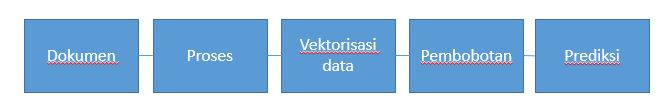
\includegraphics[width=1\textwidth]{figures/huda/chapter5/1.JPG}}
	\caption{Ilustrasi Soal No. 1}
	\label{c5_1}
\end{figure}
\item Jelaskan Mengapa dimensi dari vektor dataset google bisa mencapai 300 lengkapi dengan ilustrasi gambar.
\subitem Dimensi dari vektor dataset google bisa mencapai 300 karena dimensi dari vektor digunakan untuk membandingkan bobot dari setiap kata, misalkan terdapat kata mobil dan motor pada dataset google tersebut setiap kata tersebut di buat dimensi vektor 300 untuk kata mobil dan 300 dimensi vektor juga untuk kata motor kemudian kata tersebut di bandingkan bobot kesamaan katanya maka akan muncul akurasi sekitar 70an persen kesamaan bobot dikarenakan kata mobil dan motor sama sama di gunakan sebagai kendaraan.
\par Untuk ilustrasinya dapat dilihat pada gambar \ref{c5_2}
\begin{figure}[ht]
	\centerline{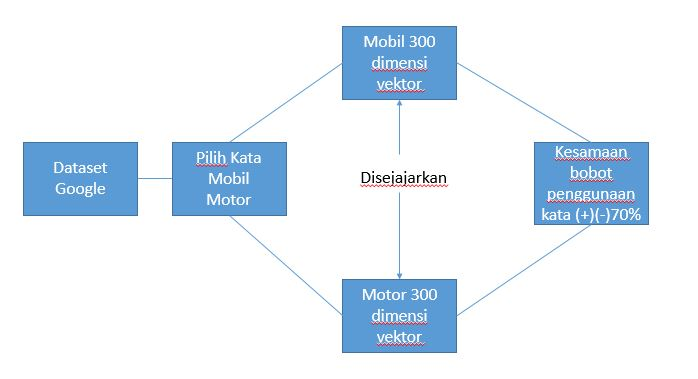
\includegraphics[width=1\textwidth]{figures/huda/chapter5/2.JPG}}
	\caption{Ilustrasi Soal No. 2}
	\label{c5_2}
\end{figure}
\item Jelaskan Konsep vektorisasi untuk kata . dilengkapi dengan ilustrasi atau gambar.
\subitem Konesp vektorisasi untuk kata yaitu mengetahui kata tengah dari suatu kalimat utama dengan suatu kalimat contoh ( Jangan lupa like dan comment yah makasih ) kata tengah tersebut merupakan (dan) yang memiliki bobot sebagai kata tengah dari suatu kalimat atau bobot sebagai objek dari suatu kalimat. hal ini sangat berkaitan dengan dimensi vektor pada dataset google yang 300 tadi karena untuk mendapatkan nilai atau bobot dari kata tengah tersebut di dapatkan dari proses dimensiasi dari kata tersebut. 
\par Untuk ilustrasinya dapat dilihat pada gambar \ref{c5_3}
\begin{figure}[ht]
	\centerline{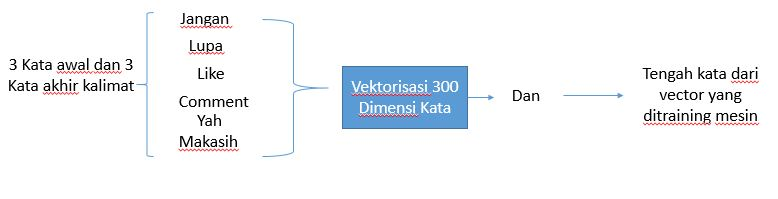
\includegraphics[width=1\textwidth]{figures/huda/chapter5/3.JPG}}
	\caption{Ilustrasi Soal No. 3}
	\label{c5_3}
\end{figure}
\item Jelaskan Konsep vektorisasi untuk dokumen. dilengkapi dengan ilustrasi atau gambar.
\subitem Konsep vektorisasi untuk dokumen hampir sama seperti vektorisasi untuk kata hanya saja pemilihan kata utama atau kata tengah terdapat pada satu dokumen jadi mesin akan membuat dimensi vektor 300 untuk dokumen dan nanti kata tengahnya akan di sandingkan pada dokumen yang terdapat pada dokumen tersebut.
\par Untuk ilustrasinya dapat dilihat pada gambar \ref{c5_4}
\begin{figure}[ht]
	\centerline{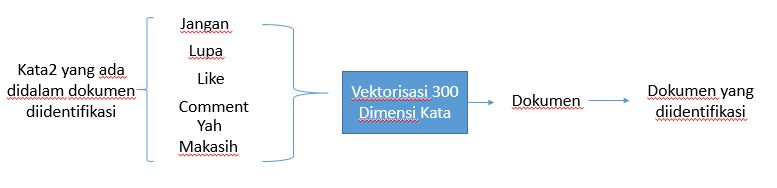
\includegraphics[width=1\textwidth]{figures/huda/chapter5/4.JPG}}
	\caption{Ilustrasi Soal No. 4}
	\label{c5_4}
\end{figure}
\item Jelaskan apa mean dan standar deviasi, lengkapi dengan iludtrasi atau gambar.
\subitem Mean adalah nilai rata-rata dari suatu data. Mean disini merupakan petunjuk terhadap kata-kata yang di olah jika kata kata itu akurasinya tinggi berarti kata tersebut sering muncul begitu juga sebaliknya. Standar deviasi merupakan standar untuk menimbang kesalahan. Misalkan kita memperkirakan kedalaman dari dataset merupakan 2 atau 3 tapi pada kenyataanya merupakan 5 itu merupakan kesalahan tapi masih bisa dianggap wajar karena masih mendekati perkiraan awal.
\par Untuk ilustrasinya dapat dilihat pada gambar \ref{c5_5}
\begin{figure}[ht]
	\centerline{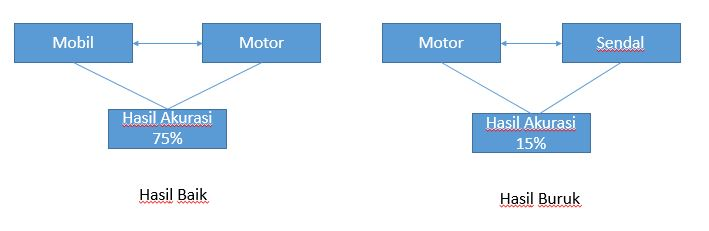
\includegraphics[width=1\textwidth]{figures/huda/chapter5/5.JPG}}
	\caption{Ilustrasi Soal No. 5}
	\label{c5_5}
\end{figure}
\item Jelaskan Apa itu Skip-Gram sertakan contoh ilustrasi.
\subitem Skip-Gram yaitu dimana kata tengah menjadi acuan terhadap kata kata pelengkap dalam suatu kalimat.
\par Untuk ilustrasinya dapat dilihat pada gambar \ref{c5_6}
\begin{figure}[ht]
	\centerline{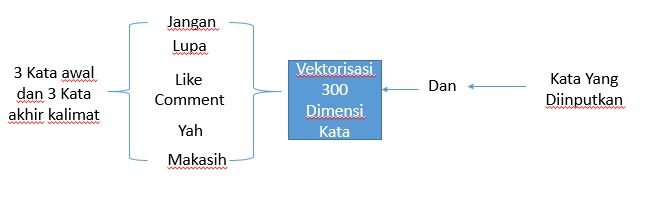
\includegraphics[width=1\textwidth]{figures/huda/chapter5/6.JPG}}
	\caption{Ilustrasi Soal No. 6}
	\label{c5_6}
\end{figure}
\end{enumerate}

\subsection{Praktek Program}
\begin{enumerate}
\item Cobalah dataset google, dan jelaskan vektor dari kata love, faith, fall, sick, clear, shine, bag, car, wash, motor, cycle dan cobalah untuk melakukan perbandingan similirati dari masing-masing kata tersebut. Jelaskan arti dari outputan similaritas.
\subitem Output source code dibawah akan memunculkan data vektor untuk kata love. bahwa vektor memiliki array sebanyak 300 dimensi. Hasil pada source code tersebut dapat dilihat pada gambar \ref{c5_7}.
\begin{verbatim}
gmodel['love']
\end{verbatim}
\begin{figure}[ht]
	\centerline{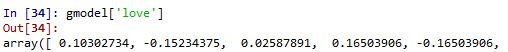
\includegraphics[width=1\textwidth]{figures/huda/chapter5/7.JPG}}
	\caption{Love}
	\label{c5_7}
\end{figure}
\subitem Output source code dibawah akan memunculkan data vektor untuk kata faith. bahwa vektor memiliki array sebanyak 300 dimensi. Hasil pada source code tersebut dapat dilihat pada gambar \ref{c5_8}.
\begin{verbatim}
gmodel['faith']
\end{verbatim}
\begin{figure}[ht]
	\centerline{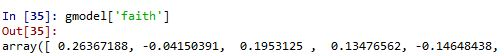
\includegraphics[width=1\textwidth]{figures/huda/chapter5/8.JPG}}
	\caption{Faith}
	\label{c5_8}
\end{figure}
\subitem Output source code dibawah akan memunculkan data vektor untuk kata fall. bahwa vektor memiliki array sebanyak 300 dimensi. Hasil pada source code tersebut dapat dilihat pada gambar \ref{c5_9}.
\begin{verbatim}
gmodel['fall']
\end{verbatim}
\begin{figure}[ht]
	\centerline{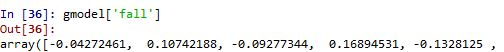
\includegraphics[width=1\textwidth]{figures/huda/chapter5/9.JPG}}
	\caption{Fall}
	\label{c5_9}
\end{figure}
\subitem Output source code dibawah akan memunculkan data vektor untuk kata sick. bahwa vektor memiliki array sebanyak 300 dimensi. Hasil pada source code tersebut dapat dilihat pada gambar \ref{c5_10}.
\begin{verbatim}
gmodel['sick']
\end{verbatim}
\begin{figure}[ht]
	\centerline{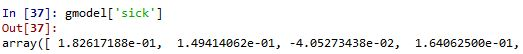
\includegraphics[width=1\textwidth]{figures/huda/chapter5/10.JPG}}
	\caption{Sick}
	\label{c5_10}
\end{figure}
\subitem Output source code dibawah akan memunculkan data vektor untuk kata clear. bahwa vektor memiliki array sebanyak 300 dimensi. Hasil pada source code tersebut dapat dilihat pada gambar \ref{c5_11}.
\begin{verbatim}
gmodel['clear']
\end{verbatim}
\begin{figure}[ht]
	\centerline{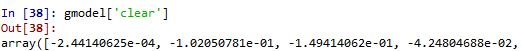
\includegraphics[width=1\textwidth]{figures/huda/chapter5/11.JPG}}
	\caption{Clear}
	\label{c5_11}
\end{figure}
\subitem Output source code dibawah akan memunculkan data vektor untuk kata shine. bahwa vektor memiliki array sebanyak 300 dimensi. Hasil pada source code tersebut dapat dilihat pada gambar \ref{c5_12}.
\begin{verbatim}
gmodel['shine']
\end{verbatim}
\begin{figure}[ht]
	\centerline{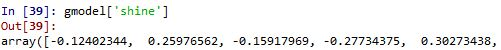
\includegraphics[width=1\textwidth]{figures/huda/chapter5/12.JPG}}
	\caption{Shine}
	\label{c5_12}
\end{figure}
\subitem Output source code dibawah akan memunculkan data vektor untuk kata bag. bahwa vektor memiliki array sebanyak 300 dimensi. Hasil pada source code tersebut dapat dilihat pada gambar \ref{c5_13}.
\begin{verbatim}
gmodel['bag']
\end{verbatim}
\begin{figure}[ht]
	\centerline{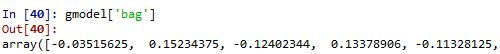
\includegraphics[width=1\textwidth]{figures/huda/chapter5/13.JPG}}
	\caption{Bag}
	\label{c5_13}
\end{figure}
\subitem Output source code dibawah akan memunculkan data vektor untuk kata car. bahwa vektor memiliki array sebanyak 300 dimensi. Hasil pada source code tersebut dapat dilihat pada gambar \ref{c5_14}.
\begin{verbatim}
gmodel['car']
\end{verbatim}
\begin{figure}[ht]
	\centerline{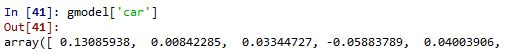
\includegraphics[width=1\textwidth]{figures/huda/chapter5/14.JPG}}
	\caption{Car}
	\label{c5_14}
\end{figure}
\subitem Output source code dibawah akan memunculkan data vektor untuk kata wash. bahwa vektor memiliki array sebanyak 300 dimensi. Hasil pada source code tersebut dapat dilihat pada gambar \ref{c5_15}.
\begin{verbatim}
gmodel['wash']
\end{verbatim}
\begin{figure}[ht]
	\centerline{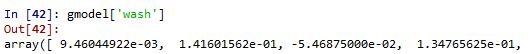
\includegraphics[width=1\textwidth]{figures/huda/chapter5/15.JPG}}
	\caption{Wash}
	\label{c5_15}
\end{figure}
\subitem Output source code dibawah akan memunculkan data vektor untuk kata motor. bahwa vektor memiliki array sebanyak 300 dimensi. Hasil pada source code tersebut dapat dilihat pada gambar \ref{c5_16}.
\begin{verbatim}
gmodel['motor']
\end{verbatim}
\begin{figure}[ht]
	\centerline{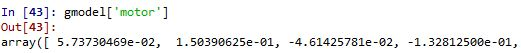
\includegraphics[width=1\textwidth]{figures/huda/chapter5/16.JPG}}
	\caption{Motor}
	\label{c5_16}
\end{figure}
\subitem Output source code dibawah akan memunculkan data vektor untuk kata cycle. bahwa vektor memiliki array sebanyak 300 dimensi. Hasil pada source code tersebut dapat dilihat pada gambar \ref{c5_17}.
\begin{verbatim}
gmodel['cycle']
\end{verbatim}
\begin{figure}[ht]
	\centerline{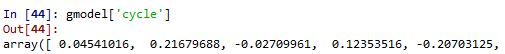
\includegraphics[width=1\textwidth]{figures/huda/chapter5/17.JPG}}
	\caption{Cycle}
	\label{c5_17}
\end{figure}
\subitem Pada source code dibawah menunjukkan hasil score perbandingan kata apakah kata motor dan cycle memiliki ke samaan atau tidak.  Hasil pada source code tersebut dapat dilihat pada gambar \ref{c5_18}.
\begin{verbatim}
gmodel.similarity('motor','cycle')
\end{verbatim}
\begin{figure}[ht]
	\centerline{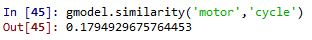
\includegraphics[width=1\textwidth]{figures/huda/chapter5/18.JPG}}
	\caption{Similariti Pada Kata Motor dan Cycle}
	\label{c5_18}
\end{figure}
\subitem Pada source code dibawah menunjukkan hasil score perbandingan kata apakah kata wash dan motor memiliki ke samaan atau tidak.  Hasil pada source code tersebut dapat dilihat pada gambar \ref{c5_19}.
\begin{verbatim}
gmodel.similarity('wash','motor')
\end{verbatim}
\begin{figure}[ht]
	\centerline{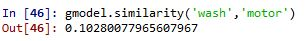
\includegraphics[width=1\textwidth]{figures/huda/chapter5/19.JPG}}
	\caption{Similariti Pada Kata Wash dan Motor}
	\label{c5_19}
\end{figure}
\subitem Untuk Motor dan Cycle hasilnya adalah 17\%
\subitem Untuk Wash dan Motor hasilnya adalah 10\%
\subitem Artinya Motor dan Cyle memang dalam kategori yang sama misalnya dalam kategori kata-kata yang disatukan/berpasangan. Mesin sudah mengetahui bahwa keduanya dapat dikategorikan sebagai sepasang kata.
\item Jelaskan dengan kata dan ilustrasi fungsi dari extract\_words dan PermuteSentences.
\subitem Extract\_Words merupakan function untuk menambahkan, menghilangkan atau menghapuskan, hal hal yang tidak penting atau tidak perlu di dalam teks. Pada gambar \ref{c5_20} berikut ini menggunakan function extract\_words untuk menghapus komen dengan python style , mencari data yang diinginkan, dan memberikan spasi pada teks.
\begin{figure}[ht]
	\centerline{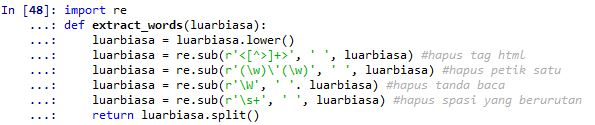
\includegraphics[width=1\textwidth]{figures/huda/chapter5/20.JPG}}
	\caption{Extract\_Words}
	\label{c5_20}
\end{figure}
\subitem PermuteSentences berfungsi untuk melakukan pengacakan data supaya memperoleh data yang teratur. Ini merupakan class yang digunakan untuk melakukan pengocokan secara acak pada data yang ada. Digunakan cara ini agar tidak terjadi kelebihan memori pada saat dijalankan. Hasilnya dapat dilihat pada gambar \ref{c5_21}.
\begin{figure}[ht]
	\centerline{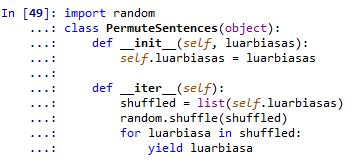
\includegraphics[width=1\textwidth]{figures/huda/chapter5/21.JPG}}
	\caption{Permute Sentences}
	\label{c5_21}
\end{figure}
\end{enumerate}